\ifx\wholebook\relax\else
\documentclass[twoside]{book}
\usepackage[active]{srcltx}
\usepackage[LY1]{fontenc}
\usepackage{epsfig}
\def\etc{{\it etc}}
\def\eg{{\it e.g.}}
\def\ie{{\it i.e.}}
\def\cf{{\it c.f.}\ }
\def\erf{\mathop{\rm erf}}
\def\sign{\mathop{\rm sign}}
\def\prob{\mathop{\rm Prob}}
\def\var{\mathop{\rm var}}
\def\mod{\mathop{\rm mod}}
\def\cor{\mathop{\rm cor}}
\def\cov{\mathop{\rm cov}}
\def\cl{\mathop{\rm CL}}
\def\kg{\mathop{\rm Kg}}
\def\patstyle#1{{\sc #1}}
\def\th{^{\mathop{\rm th}}}
\def\st#1{^{\mathop{\rm #1}}}
\def\note#1{\begin{quote}{\bf Note:} #1\end{quote}}
\def\braket#1{\left\langle #1\right\rangle}
\def\order#1{\let\o=#1{\cal O}\ifx\o 1$\left(n\right)$\else$\left(n^{#1}\right)$\fi}
\newtheorem{privListing}{Listing}[chapter]
\newenvironment{listing}{\vskip 3ex\hrule\vskip 1ex\begin{privListing}}{\end{privListing}\hrule\vskip 1ex}
\newtheorem{privExample}{Code example}[chapter]
\newenvironment{codeExample}{\begin{privExample}\begin{quote}\tt}{\end{quote}\end{privExample}}
\def\relboxl#1#2{\hbox to #1\hsize{#2\hfil}}
\def\relboxc#1#2{\hbox to #1\hsize{\hfil #2\hfil}}
\def\relboxr#1#2{\hbox to #1\hsize{\hfil #2}}
\def\transpose#1{{\bf #1}^{\mathop{\rm T}}}
\def\inverse#1{{\bf #1}^{-1}}
%\def\tm{$^{\mathop{\rm TM}}$}
\def\tm{ }
\newenvironment{mainEquation}{\marginpar[\vspace{3 ex} Main
equation$\Rightarrow$]{\vspace{3 ex}$\Leftarrow$Main
equation}\begin{equation}}{\end{equation}}
\def\rubrique#1{\paragraph{#1}\hfil\par\noindent}

\begin{document}
\fi

\chapter{Integration of functions}
\label{ch:integration}
\begin{flushright}
{\sl Les petits ruisseaux font les grandes
rivi\`{e}res}\footnote{Small streams build great rivers.}\\ French
proverb
%If quote is changed, introduction must be changed
\end{flushright}
\vspace{1 ex}Many functions are defined by an integral. For
example, the three functions discussed in the last 3 sections of
chapter \ref{ch:function} were all defined by an integral. When no
other method is available the only way to compute such function is
to evaluate the integral. Integrals are also useful in probability
theory to compute the probability of obtaining a value over a
given interval. This aspect will be discussed in chapter
\ref{ch:statistics}. Finally integrals come up in the computation
of surfaces and of many physical quantities related to energy and
power. For example, the power contained in an electromagnetic
signal is proportional to the integral of the square of the
signal's amplitude.

The French proverb quoted at the beginning of this chapter is here
to remind people that an integral is defined formally as the
infinite sum of infinitesimal quantities.

\section{Introduction}
Let us begin with a concrete example. This time we shall take a
problem from physics 101.

When light is transmitted through a narrow slit, it is diffracted.
The intensity of the light transmitted at an angle $\vartheta$,
$I\left(\vartheta\right)$, is given by:
\begin{equation}
  I\left(\vartheta\right)={\sin^2\vartheta \over \vartheta^2}
\end{equation}
If one wants to compute the fraction of light which is transmitted
within the first diffraction peak, one must compute the
expression:
\begin{equation}
\label{eq:intensity}
  I\left(\vartheta\right)={1 \over\pi}\int_{-\pi}^{\pi}{\sin^2\vartheta \over
  \vartheta^2}d\vartheta.
\end{equation}
The division by $\pi$ is there because the integral of
$I\left(\vartheta\right)$ from $-\infty$ to $+\infty$ is equal to
$\pi$. No closed form exists for the integral of equation
\ref{eq:intensity}: it must be computed numerically. This answer
is $90.3\%$.

In this chapter we introduce 3 integration algorithms. Figure
\ref{fig:integclass} shows the corresponding class diagram.
\begin{figure}
\centering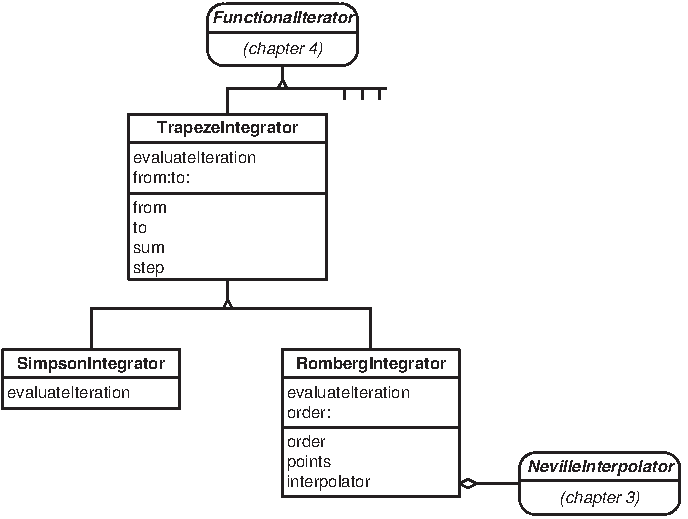
\includegraphics[width=10cm]{Figures/IntegrationClassDiagram}
\caption{Class diagram of integration
classes}\label{fig:integclass}
\end{figure}
The first one, trapeze integration, is only introduced for the
sake of defining a common framework for the next two algorithms:
Simpson and Romberg integration. In general, the reader should use
Romberg's algorithm. It is fast and very precise. There are,
however, some instances where Simpson's algorithm can be faster if
high accuracy is not required.

\section{General framework --- Trapeze integration method}
\label{sec:trapeze} Let us state it at the beginning. One should
not use the trapeze integration algorithm in practice. The
interest of this algorithm is to define a general framework for
numerical integration. All subclasses of the class responsible for
implementing the trapeze integration algorithm will reuse most the
mechanisms described in this section.

The trapeze numerical integration method takes its origin in the
series expansion of an integral. This series expansion is
expressed by the Euler-Maclaurin formula shown hereafter
\cite{Bass}:
\begin{equation}
\label{eq:eulerMacLaurin}
  \int_a^b f\left(x\right)dx={b-a\over
  2}\left[f\left(a\right)+f\left(b\right)\right]-\sum_n{\left(b-a\right)^2\over
  \left(2n\right)!}B_{2n}\left[{d^{2n-1}f\left(b\right)\over dx^{2n-1}}-{d^{2n-1}f\left(a\right)\over
  dx^{2n-1}}\right],
\end{equation}
where the numbers $B_{2n}$ are the Bernouilli numbers.

The next observation is that, if the interval of integration is
small enough, the series in the second term of equation
\ref{eq:eulerMacLaurin} would yield a contribution negligible
compared to that of the first term. Thus, we can write:
\begin{equation}
\label{eq:approxEML}
  \int_a^b f\left(x\right)dx\approx{b-a\over
  2}\left[f\left(a\right)+f\left(b\right)\right],
\end{equation}
if $b-a$ is sufficiently small. The approximation of equation
\ref{eq:approxEML} represents the area of a trapeze whose summits
are the circled points in Figure \ref{fig:trapeze}. Finally, one
must remember the additive formula between integrals:
\begin{figure}
\centering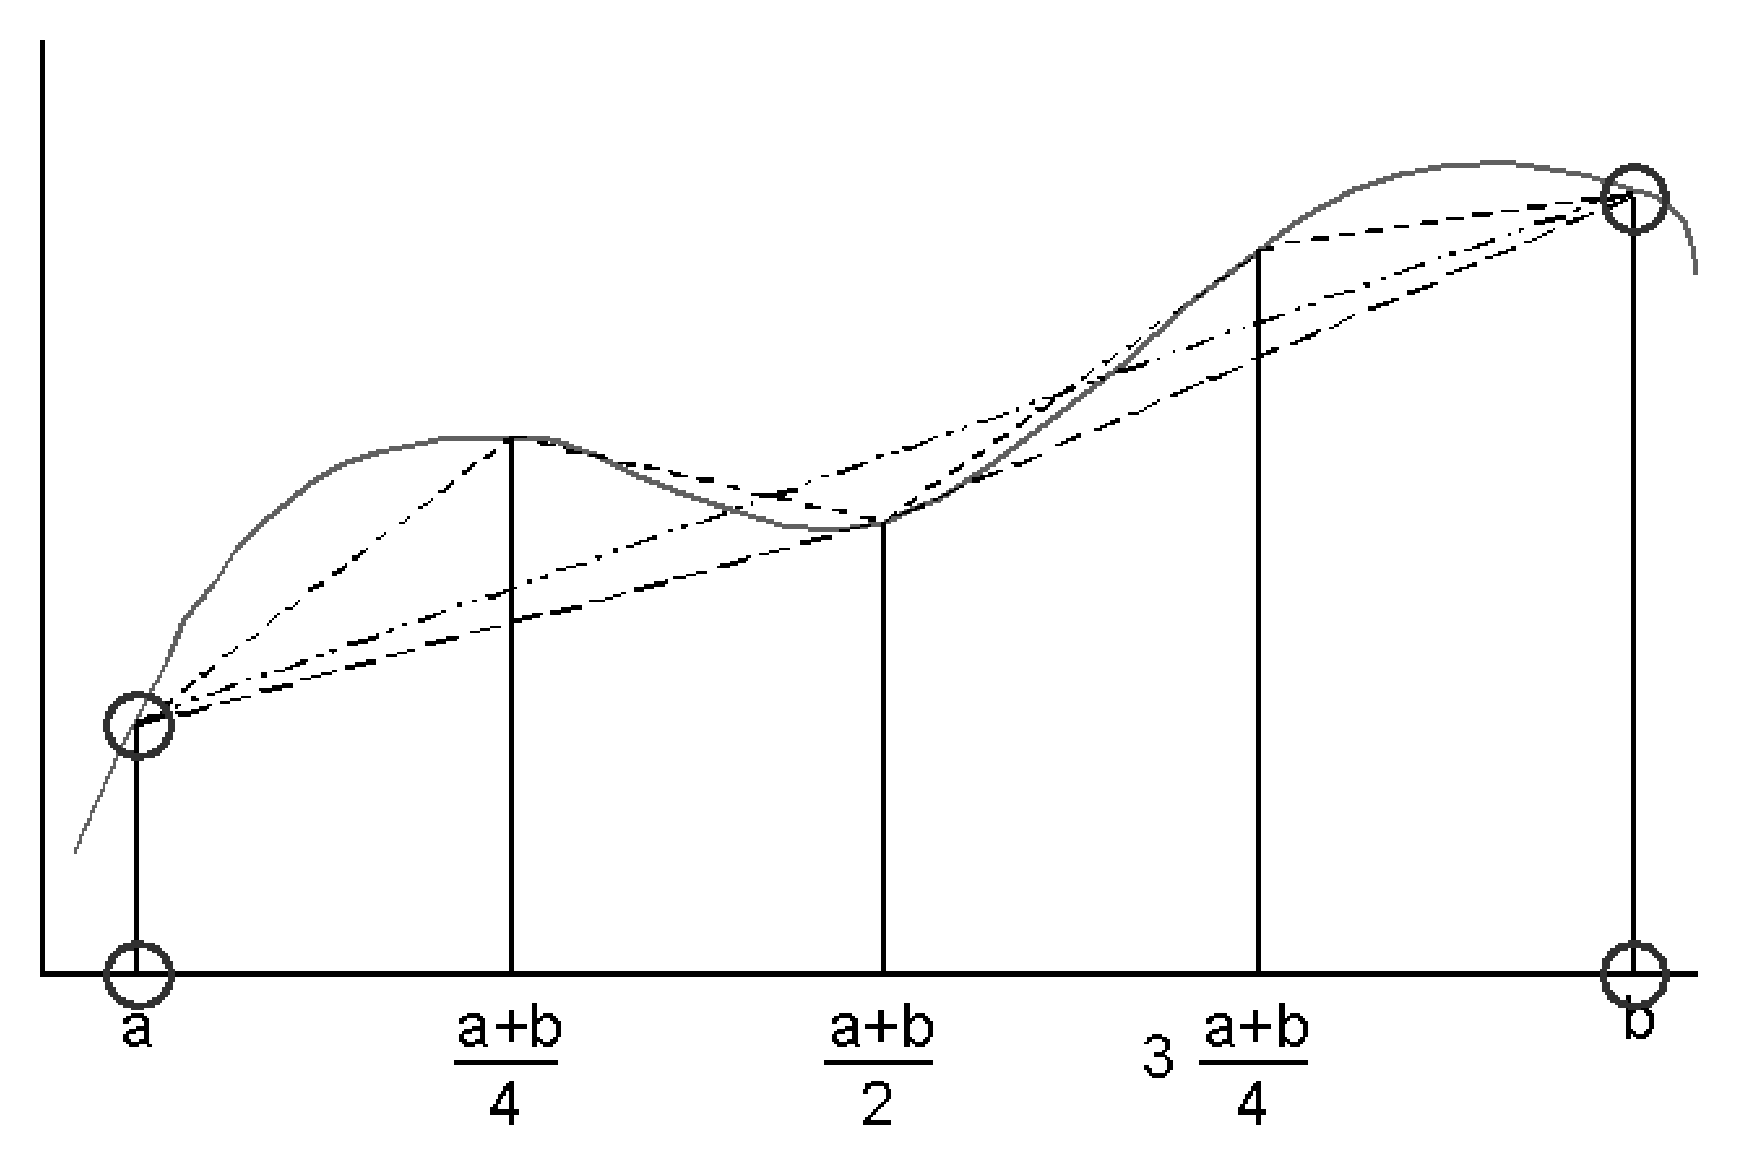
\includegraphics[width=10cm]{Figures/IntegrationGraph}
\caption{Geometrical interpretation of the trapeze integration
method}\label{fig:trapeze}
\end{figure}
\begin{equation}
\label{eq:addintegral}
  \int_a^b f\left(x\right)dx=\int_a^c f\left(x\right)dx+\int_c^b f\left(x\right)dx,
\end{equation}
for any $c$. We shall use this property by chosing a $c$ located
between $a$ and $b$.

The resulting strategy is a divide-and-conquer strategy. The
integration interval is divided until one can be sure that the
second term of equation \ref{eq:eulerMacLaurin} becomes indeed
negligible. As one would like to re-use the points at which the
function has been evaluated during the course of the algorithm,
the integration interval is halved at each iteration. The first
few steps are outlined in figure \ref{fig:trapeze}. An estimation
of the integral is obtained by summing the areas of the trapezes
corresponding to each partition.

Let $x_0^{\left(n\right)},\ldots,x_{2^n}^{\left(n\right)}$ be the
partition of the interval at iteration $n$. Let
$\epsilon^{\left(n\right)}$ be the length of each interval between
these points. We thus have:
\begin{equation}
  \left\{
  \begin{array}{lcl}
    \epsilon^{\left(n\right)} & = & {\displaystyle b-a \over\displaystyle 2^n} \\
    x_0^{\left(n\right)} & = & a \\*[0.5ex]
    x_i^{\left(n\right)} & = & a+i\epsilon^{\left(n\right)}
    \mbox{\quad for $i=1,\ldots,2^n$.}
  \end{array}
  \right.
\end{equation}
The corresponding estimation for the integral is:
\begin{equation}
\label{eq:trapezesum}I^{\left(n\right)}=\epsilon^{\left(n\right)}\left[f\left(a\right)+f\left(b\right)+2
\sum_{i=1}^{2^n-1}f\left(x_i^{\left(n\right)}\right)\right] .
\end{equation}
To compute the next estimation, it suffices to compute the value
of the function at the even values of the partition because the
odd values were already computed before. One can derive the
following recurrence relation:
\begin{mainEquation}
\label{eq:trapeze} I^{\left(n+1\right)}={I^{\left(n\right)}\over
2}+ \epsilon^{\left(n\right)}
\sum_{i=1}^{2^n-1}f\left(x_{2i-1}^{\left(n\right)}\right),
\end{mainEquation}
with the initial condition:
\begin{equation}
I^{\left(0\right)}={b-a \over
2}\left[f\left(a\right)+f\left(b\right)\right].
\end{equation}
Note that the sum on the right-hand side of equation
\ref{eq:trapeze} represents the sum of the function's values at
the new points of the partition.

\rubrique{End game strategy} The final question is when should the
algorithm be stopped? A real honest answer is we do not know. The
magnitude of the series in equation \ref{eq:eulerMacLaurin} is
difficult to estimate as the Bernouilli numbers become very large
with increasing $n$. An experimental way is to watch for the
change of the integral estimate In other words the absolute value
of the last variation,
$\left|I^{\left(n\right)}-I^{\left(n+1\right)}\right|$ , is
considered a good estimate of the precision. This kind of
heuristic works for most functions.

At each iteration the number of function evaluation doubles. This
means that the time spent in the algorithm grows exponentially
with the number of iterations. Thus, the default maximum number of
iteration must be kept quite low compared to that of the other
methods.

In practice, however, trapeze integration converges quite slowly
and should not be used. Why bother implementing it then? It turns
out that the more elaborate methods, Simpson and Romberg
integration, require the computation of the same sums needed by
the trapeze integration. Thus, the trapeze integration is
introduced to be the superclass of the other better integration
methods.

One must keep in mind, however, that the magnitude of the series
in equation \ref{eq:eulerMacLaurin} can become large for any
function whose derivatives of high orders have singularities over
the interval of integration. The convergence of the algorithm can
be seriously compromised for such functions. This remark is true
for the other algorithms described in this chapter. For example,
none of the algorithms is able to give a precise estimate of the
beta function using equation \ref{eq:betaint} with $x>1$ and $y<1$
(\cf section \ref{sec:betafunc}) because, for these values, the
derivatives of the function to integrate have a singularity at
$t=1$.

Another problem can come up if the function is nearly zeroes at
regular intervals. For example, evaluating the integral of the
function $f\left(x\right)={\sin\left(2^mx\right)\over x}$  from
$-\pi$ to $\pi$ for a moderate value of $m$. In this case, the
terms $I^{\left(0\right)}$ to $I^{\left(m\right)}$ will have a
null contribution. This would cause the algorithm to stop
prematurely. Such special function behavior is of course quite
rare. Nevertheless the reader must be aware of the limitations of
the algorithm. This remark is valid for all algorithms exposed in
this chapter.

\subsection{Trapeze integration --- General implementation}
\marginpar{Figure \ref{fig:integclass} with the box {\bf
TrapezeIntegrator} grayed.}The class implementing trapeze
integration is a subclass of the functional iterator discussed in
section \ref{sec:iterrel}. Two instance variables are needed to
define the integration interval. Additional instance variables
must keep track of the partition of the interval and of the
successive estimations. Consequently, the class has the following
instance variables.
\begin{description}
\item[\tt from] contains the lower limit of the integration's interval,
 \ie\ $a$.
\item[\tt to] contains the lower limit of the integration's interval,
 \ie\ $b$.
\item[\tt step] contains the size of the interval's partition,
 \ie\ $\epsilon^{\left(n\right)}$.
\item[\tt sum] contains the intermediate sums, \ie\ $I^{\left(n\right)}$.
\end{description}

Although trapeze integration is not a practical algorithm, we give
an example of coding for both language implementations. The reason
is that the public interface used by trapeze integration is the
same for all integration classes.

The example shown in the next two sections is the integration of
the inverse function. In mathematics the natural logarithm of $x$,
$\ln x$, is defined as the integral from 1 to $x$ of the inverse
function. Of course, using numerical integration is a very
inefficient way of computing a logarithm. This example, however,
allows the reader to investigate the accuracy (since the exact
solution is known) and performances of all algorithms presented in
this chapter. The interested reader should try the example for
various setting of the desired precision and look at the number of
iterations needed for a desired precision. She can also verify how
accurate is the estimated precision.

\subsection{Trapeze integration --- Smalltalk implementation}
\label{sec:strapeze} Listing \ref{ls:trapeze} shows the Smalltalk
implementation of the trapeze integration method. In Smalltalk the
code for the computation of the integral defining the natural
logarithm is as follows:
\begin{codeExample}
\begin{verbatim}

\end{verbatim}
{\tt | integrator ln2 ln3 |}\\ {\tt integrator :=
DhbTrapezeIntegrator function: [ :x | 1.0 / x ] from: 1 to: 2.}\\
{\tt ln2 := integrator evaluate.}\\ {\tt integrator from: 1 to:
3.}\\ {\tt ln3 := integrator evaluate.}\\
\end{codeExample}
The line after the declaration creates a new instance of the class
{\tt DhbTrapezeIntegrator} for the inverse function. The limits of
the integration interval are set from 1 to 2 at creation time. The
third line retrieves the value of the integral. The fourth line
changes the integration interval and the last line retrieves the
value of the integral over the new integration interval.

The class {\tt DhbTrapezeIntegrator} is a subclass of the class
{\tt AbstractFunctionIterator} defined in section
\ref{sec:siterrel}. The default creation class method {\tt new}
has been overloaded to prevent creating an object without
initialized instance variables. The proper creation class method
defines the function and the integration interval.

The method {\tt from:to:} allows changing the integration interval
for a new computation with the same function.

Note that the initialization of the iterations (method {\tt
computeInitialValues}, \cf section \ref{sec:siteration}) also
corresponds to the first iteration of the algorithm. The method
{\tt highOrderSum} computes the sum of the right-hand side of
equation \ref{eq:trapeze}.

\begin{listing} Smalltalk implementation of trapeze integration
\label{ls:trapeze}
$$\halign{ #\hfil&\quad#\hfil\cr {\sl Class}& {\Large\bf DhbTrapezeIntegrator}\cr
{\sl Subclass of }&{\tt DhbFunctionalIterator}\cr\noalign{\vskip 1ex}

{\sl Instance variable names:}&\parbox[t]{4 in}{\tt  from to sum step }\cr\noalign{\vskip 1ex}}$$


Class methods
{\parskip 1ex\par\noindent}
{\bf defaultMaximumIterations}
\begin{verbatim}
    ^13

\end{verbatim}
{\bf new}
\begin{verbatim}
    ^self error: 'Method new:from:to: must be used'

\end{verbatim}
{\bf new:} {\tt aBlock} {\bf from:} {\tt aNumber1} {\bf to:} {\tt aNumber2}
\begin{verbatim}
    ^super new initialize: aBlock from: aNumber1 to: aNumber2

\end{verbatim}



Instance methods
{\parskip 1ex\par\noindent}
{\bf computeInitialValues}
\begin{verbatim}
    step := to - from.
    sum := ( ( functionBlock value: from) + ( functionBlock value: 
                                                       to)) * step /2.
    result := sum.

\end{verbatim}
{\bf evaluateIteration}
\begin{verbatim}
    | oldResult |
    oldResult := result.
    result := self higherOrderSum.
    ^self relativePrecision: ( result - oldResult) abs

\end{verbatim}
{\bf from:} {\tt aNumber1} {\bf to:} {\tt aNumber2}
\begin{verbatim}
    from := aNumber1.
    to := aNumber2.

\end{verbatim}
{\bf higherOrderSum}
\begin{verbatim}
    | x newSum |
    x := step / 2 + from.
    newSum := 0.
    [ x < to ]
        whileTrue: [ newSum := ( functionBlock value: x) + newSum.
                     x := x + step.
                   ].
    sum := ( step * newSum + sum) / 2.
    step := step / 2.
    ^sum

\end{verbatim}
{\bf initialize:} {\tt aBlock} {\bf from:} {\tt aNumber1} {\bf to:} {\tt aNumber2}
\begin{verbatim}
    functionBlock := aBlock.
    self from: aNumber1 to: aNumber2.
    ^self   

\end{verbatim}


\end{listing}


\section{Simpson integration algorithm}
\marginpar{Figure \ref{fig:integclass} with the box {\bf
SimpsonIntegrator} grayed.}Simpson integration algorithm consists
in replacing the function to integrate by a second order Lagrange
interpolation polynomial\cite{Bass} (\cf section
\ref{sec:lagrange}). One can then carry the integral analytically.
Let $f\left(x\right)$ be the function to integrate. For a given
interval of integration, $\left[a,b\right]$, the function is
evaluated at the extremities of the interval and at its middle
point $c={a+b \over 2}$. As defined in equation \ref{eq:lagrange}
the second order Lagrange interpolation polynomial is then given
by:
\begin{equation}
  P_2\left(x\right)={2\over \left(b-a\right)^2}\left[\left(x-b\right)\left(x-c\right)f\left(a\right) +\left(x-c\right)\left(x-a\right)f\left(b\right) +
  \left(x-a\right)\left(x-b\right)f\left(c\right)\right].
\end{equation}
The integral of the polynomial over the interpolation interval is
given by:
\begin{equation}
\label{eq:simpson} \int_a^b P_2\left(x\right)dx={b-a \over
6}\left[f\left(a\right) + f\left(b\right) + 4 f\left(c\right)
\right].
\end{equation}
As for trapeze integration, the interval is partitioned into small
intervals. Let us assume that the interval has been divided into
subintervals. By repeating equation \ref{eq:simpson} over each
subinterval, we obtain:
\begin{equation}
\label{eq:simpsum} \int_a^b
P_2\left(x\right)dx={\epsilon^{\left(n\right)} \over
3}\left[f\left(a\right) + f\left(b\right) + 2 \sum_{i=1}^{2^{n-1}}
f\left(x_{2i-1}^{\left(n\right)}\right) + 4 \sum_{i=0}^{2^{n-1}}
f\left(x_{2i}^{\left(n\right)}\right) \right].
\end{equation}
Equation \ref{eq:simpsum} uses the notations introduced in section
\ref{sec:trapeze}. Except for the first iteration, the right-hand
side of equation \ref{eq:simpsum} can be computed from the
quantities $I^{\left(n\right)}$ defined in equation
\ref{eq:trapezesum}. Thus, we have:
\begin{mainEquation}
  \int_a^b
P_2\left(x\right)dx={1 \over
3}\left[4I^{\left(n\right)}-I^{\left(n-1\right)}\right]
\mbox{\quad for $n>1$}
\end{mainEquation}
This can be checked by verifying that $I^{\left(n-1\right)}$ is
equal to the first sum of equation \ref{eq:simpsum} times  and
that $I^{\left(n\right)}$  is equal to the addition of the two
sums of equation \ref{eq:simpsum} times
$\epsilon^{\left(n\right)}$. As advertised in section
\ref{sec:trapeze} we can re-use the major parts of the trapeze
algorithm: computation of the sums and partition of the
integration interval.

Like in the case of the trapeze algorithm, the precision of the
algorithm is estimated by looking at the differences between the
estimation obtained previously and the current estimation. At the
first iteration only one function point is computed. This can
cause the process to stop prematurely if the function is nearly
zero at the middle of the integration interval. Thus, a protection
must be built in to prevent the algorithm from stopping at the
first iteration.

\subsection{Simpson integration --- General implementation}
The class implementing Simpson algorithm is a subclass of the
class implementing trapeze integration. The method {\tt
evaluateIteration} is the only method needing change. The number
of iterations is checked to prevent returning after the first
iteration.

The public interface is the same as that of the superclass. Thus,
all the examples shown in sections \ref{sec:strapeze} and
\ref{sec:jtrapeze} can be used for Simpson algorithm by just
changing the name of the class.

\subsection{Simpson integration --- Smalltalk implementation}
\label{sec:sSimpson} Listing \ref{ls:simpson} shows the complete
implementation in Smalltalk.

The class {\tt DhbSimpsonIntegrator} is a subclass of the class
{\tt DhbTrapezeIntegrator} defined in section \ref{sec:strapeze}.

\begin{listing} Smalltalk implementation of the Simpson integration algorithm \label{ls:simpson}
$$\halign{ #\hfil&\quad#\hfil\cr {\sl Class}& {\Large\bf DhbSimpsonIntegrator}\cr
{\sl Subclass of }&{\tt DhbTrapezeIntegrator}\cr\noalign{\vskip 1ex}
}$$


Instance methods
{\parskip 1ex\par\noindent}
{\bf evaluateIteration}
\begin{verbatim}
    | oldResult oldSum |
    iterations < 2
        ifTrue: [ self higherOrderSum.
                  ^1
                ].
    oldResult := result.
    oldSum := sum.
    result := (self higherOrderSum * 4 - oldSum) / 3.
    ^self relativePrecision: ( result - oldResult) abs

\end{verbatim}


\end{listing}


\section{Romberg integration algorithm}
\label{sec:romberg}\marginpar{Figure \ref{fig:integclass} with the
box {\bf RombergIntegrator} grayed.} If one goes back to equation
\ref{eq:eulerMacLaurin} one notices that the second term is of the
order of the square of the integration interval. Romberg's
algorithm uses this fact to postulate that $I^{\left(n\right)}$ is
a smooth function of the square of the size of interval's
partition $\epsilon^{\left(n\right)}$. Romberg's algorithm
introduces the parameter $k$ where $k-1$ is the degree of the
interpolation's polynomial\footnote{In other words, $k$ is the
number of points over which the interpolation is performed (\cf
section \ref{sec:lagrange}).}. The result of the integral is
estimated by extrapolating the series
$I^{\left(n-k\right)},\ldots,I^{\left(n\right)}$ at the value
$\epsilon^{\left(n\right)}=0$. Since we have:
\begin{equation}
\epsilon^{\left(n\right)}={\epsilon^{\left(n-1\right)} \over 2},
\end{equation}
one only needs to interpolate over successive powers of $1/4$ ,
starting with 1: 1, $1/4$, $1/16$, $1/256$, \etc. In this case,
extrapolation is safe because the value at which extrapolation is
made is very close to the end of the interval defined by the
sample points and actually becomes closer and closer with every
iteration.

Thus, Romberg's algorithm requires at least $k$ iterations. The
good news is that this algorithm converges very quickly and, in
general, only a few iterations are needed after the five initial
ones. A polynomial of $4^{\mathop{\rm th}}$ degree --- that is
$k=5$ --- is generally sufficient \cite{Press}.

Extrapolation is performed using Neville's algorithm (\cf section
\ref{sec:neville}) because it computes an estimate of the error on
the interpolated value. That error estimate can then be used as
the estimate of the error on the final result.

If $k=1$ Romberg's algorithm is equivalent to trapeze integration.
If $k=2$, the interpolation polynomial is given by:
\begin{equation}
P_1\left(x\right)=y_1+{x-x_1 \over x_2-x_1}\left(y_2-y_1\right).
\end{equation}
At the $n^{\mathop{\rm th}}$ iteration we have:
$y_1=I^{\left(n-1\right)}$, $y_2=I^{\left(n\right)}$ and
$x_2=x_1/4$. Thus, the interpolated value at 0 is:
\begin{equation}
P_1\left(0\right)=I^{\left(n-1\right)}+{4 \over
3}\left[I^{\left(n\right)}-I^{\left(n-1\right)}\right] ={1\over
3}\left[4I^{\left(n\right)}-I^{\left(n-1\right)}\right]
\end{equation}
Thus, for $k=2$ Romberg's algorithm is equivalent to Simpson's
algorithm. For higher order, however, Romberg's algorithm is much
more efficient than Simpson method as soon as precision is
required (\cf a comparison of the result in section
\ref{sec:intwhich}).

Using interpolation on the successive results of an iterative
process to obtain the final result is a general procedure known as
Richardson's deferred approach to the limit \cite{Press}. This
technique can be used whenever the estimated error can be
expressed as a function of a suitable parameter depending on the
iterations. The choice of the parameter, however, is critical. For
example, if one had interpolated over the size of the interval's
partition instead of its square, the method would not converge as
well\footnote{It converges at the same speed as Simpson's
algorithm. This can be verified by running the comparison programs
after changing the factor 0.25 used to compute the abscissa of the
next point into 0.5.}.

\subsection{Romberg integration --- General implementation}
The class implementing Romberg's algorithm needs the following
additional instance variables:
\begin{description}
\item[\tt order]the order of the interpolation, \ie\ $k$,\\
\item[\tt interpolator ]an instance of Neville's interpolation class,\\
\item[\tt points]an {\tt OrderedCollection} containing the most recent sum estimates,
\ie\ $I^{\left(n-k\right)},\ldots,I^{\left(n\right)}$.\\
\end{description}
The method {\tt evaluateIteration} (c.f. section
\ref{sec:iteration}) contains the entire algorithm. At each
iteration the collection of point receives a new point with an
abscissa equal to the quarter of that of the last point and an
ordinate equal to the next sum estimate . If not enough points are
available, the method returns a precision such that the iterative
process will continue. Otherwise, the extrapolation is performed.
After the result of the extrapolation has been obtained the oldest
point is removed. In other words, the collection of points is used
as a last-in-last-out list with a constant number of elements
equal to the order of the interpolation. Of the two values
returned by Neville's interpolation (\cf section
\ref{sec:neville}), the interpolated value is stored in the result
and the error estimate is returned as the precision for the other.

\subsection{Romberg integration --- Smalltalk implementation}
\label{sec:sromberg} Listing \ref{ls:romberg} shows the Smalltalk
implementation of Romberg's algorithm. The class {\tt
DhbRombergIntegrator} is a subclass of the class {\tt
DhbTrapezeIntegrator} defined in section \ref{sec:strapeze}.

The class method {\tt defaultOrder} defines the default order to
5. This method is used in the method initialize so that each newly
created instance is created with the default interpolation order.
The method {\tt order:} allows changing the default order if
needed.

The sample points defining the interpolation are stored in an {\tt
OrderedCollection}. This collection is created in the method {\tt
computeInitialValues}. Since the number of points will never
exceed the order of the interpolation the maximum size is preset
when the collection is created. The method {\tt
computeInitialValues} also creates the object in charge of
performing the interpolation and it stores the first point in the
collection of sample points.
\begin{listing} Smalltalk implementation of Romberg integration \label{ls:romberg}
$$\halign{ #\hfil&\quad#\hfil\cr {\sl Class}& {\Large\bf DhbRombergIntegrator}\cr
{\sl Subclass of }&{\tt DhbTrapezeIntegrator}\cr\noalign{\vskip 1ex}

{\sl Instance variable names:}&\parbox[t]{4 in}{\tt  order points interpolator }\cr\noalign{\vskip 1ex}}$$


Class methods
{\parskip 1ex\par\noindent}
{\bf defaultOrder}
\begin{verbatim}
    ^5
\end{verbatim}



Instance methods
{\parskip 1ex\par\noindent}
{\bf computeInitialValues}
\begin{verbatim}
    super computeInitialValues.
    points := OrderedCollection new: order.
    interpolator := DhbNevilleInterpolator points: points.
    points add: 1 @ sum.
\end{verbatim}
{\bf evaluateIteration}
\begin{verbatim}
    | interpolation |
    points addLast: (points last x * 0.25) @ self higherOrderSum.
    points size < order
        ifTrue: [ ^1].
    interpolation := interpolator valueAndError: 0.
    points removeFirst.
    result := interpolation at: 1.
    ^self relativePrecision: ( interpolation at: 2) abs
\end{verbatim}
{\bf initialize}
\begin{verbatim}
    order := self class defaultOrder.
    ^ super initialize
\end{verbatim}
{\bf order:} {\tt anInteger}
\begin{verbatim}
    anInteger < 2
        ifTrue: [ self error: 'Order for Romberg integration must be 
                                                      larger than 1'].
    order := anInteger.
\end{verbatim}


\end{listing}

\section{Evaluation of open integrals}
An open integral is an integral for which the function to
integrate cannot be evaluated at the boundaries of the integration
interval. This is the case when one of the limit is infinite or
when the function to integrate has a singularity at one of the
limits. If the function to integrate has one or more singularity
in the middle of the integration interval, the case can be reduced
to that of having a singularity at the limits using the additive
formula between integrals \ref{eq:addintegral}. Generalization of
the trapeze algorithm and the corresponding adaptation of
Romberg's algorithm can be found in \cite{Press}.

\rubrique{Bag of tricks} My experience is that using a suitable
change of variable can often remove the problem. In particular,
integrals whose integration interval extends to infinity can be
rewritten as integrals over a finite interval. We give a few
examples below.

For an integral starting from minus infinity, a change of variable
$t={1 \over x}$ can be used as follows:
\begin{equation}
\label{eq:inftyvarchg}
  \int_{-\infty}^a f\left(x\right)dx= \int_{1\over a}^0 f\left({1\over
  t}\right){dt\over t^2}\mbox{\quad for $a<0$.}
\end{equation}
For such integral to be defined, the function must vanish at minus
infinity faster than $x^2$. This means that:
\begin{equation}
  \lim_{t \to 0}{1\over t^2}f\left({1\over
  t}\right)=0.
\end{equation}
If $a>0$, the integration must be evaluated in two steps, for
example one over the interval $\left]-\infty,-1\right]$ using the
change of variable of equation \ref{eq:inftyvarchg} and one over
the interval $\left[-1,a\right]$ using the original function.

For integral ending at positive infinity the same change of
variable can also be made. However, if the interval of integration
is positive, the change of variable $t=e^{-x}$ can be more
efficient. In this case, one makes the following transformation:
\begin{equation}
\int_a^{+\infty} f\left(x\right)dx=\int_0^{e^{-a}}f\left(-\ln t
\right){dt \over t}\mbox{\quad for $a>0$}.
\end{equation}
For this integral to be defined one must have:
\begin{equation}
  \lim_{t \to 0}{1\over t}f\left(\ln
  t\right)=0.
\end{equation}
By breaking up the interval of integration is several pieces one
can chose a change of variable most appropriate for each piece.

\section{Which method to chose?}
\label{sec:intwhich} An example comparing the results of the three
algorithms is given in section \ref{sec:sintcompar} for Smalltalk.
The function to integrate is the inverse function in both cases. The integration
interval is from 1 to 2 so that the value of the result is known,
namely $\ln 2$. Integration is carried for various values of the
desired precision. The reader can then compare the attained
precision (both predicted and real) and the number of
iterations\footnote{Note that the number of iterations printed in
the examples in one less than the real number of iterations
because the first iteration is performed in the set-up phase of
the iterative process.} required for each algorithm. Let us recall
that the number of required function evaluations grows
exponentially with the number of iterations.

The results clearly show that the trapeze algorithm is ruled out
as a practical method. As advertised in section \ref{sec:trapeze}
it is not converging quickly toward a solution.

Romberg's algorithm is the clear winner. At given precision, it
requires the least number of iterations. This is the algorithm of
choice in most cases.

Simspon's algorithm may be useful if the required precision is not
too high and if the time to evaluate the function is small
compared to the interpolation. In such cases Simspon's algorithm
can be faster than Romberg's algorithm.

Sections \ref{sec:sintcompar} and \ref{sec:jintcompar} gives some
sample code the reader can use to investigate the various
integration algorithms. The results of the code execution are
shown in table \ref{tb:intcompar}. The columns of this table are:
\begin{description}
\item[$\epsilon_{\mathop{\rm max}}$]the desired precision,\\
\item[$n$]the number of required iterations; let us recall that the
corresponding number of function's evaluations is $2^{n+1}$,\\
\item[$\tilde{\epsilon}$]the estimated precision of the result,\\
\item[$\epsilon$]the effective precision of the result, that is the absolute value
of the difference between the result of the integration algorithm and the true result.\\
\end{description}

\begin{table}[h]
  \centering
  \caption{Comparison between integration algorithms}\label{tb:intcompar}
\vspace{1 ex}
\begin{tabular}{|l|l|l|l|l|l|l|l|l|l|} \hline
  &\multicolumn{3}{c|}{\bf Trapeze algorithm} &\multicolumn{3}{c|}{\bf Simpson algorithm}&\multicolumn{3}{c|}{\bf Romberg algorithm}  \\ \hline
  $\epsilon_{\mathop{\rm max}}$ & $n$ & $\tilde{\epsilon}$ & $\epsilon$ & $n$ & $\tilde{\epsilon}$ & $\epsilon$ & $n$ & $\tilde{\epsilon}$ & $\epsilon$
  \\ \hline
$10^{-5}$&8&$4.1\cdot 10^{-6}$&$9.5\cdot 10^{-7}$&4&$9.9\cdot
10^{-6}$&$4.7\cdot 10^{-7}$&4&$1.7\cdot 10^{-9}$&$1.4\cdot
10^{-9}$\\ \hline $10^{-7}$&11&$6.4\cdot 10^{-8}$&$1.5\cdot
10^{-8}$&6&$4.0\cdot 10^{-8}$&$1.9\cdot 10^{-9}$&4&$1.7\cdot
10^{-9}$&$1.4\cdot 10^{-9}$\\ \hline $10^{-9}$ &15&$2.5\cdot
10^{-10}$&$5.8\cdot 10^{-11}$&8&$1.5\cdot 10^{-10}$&$7.3\cdot
10^{-12}$&5&$1.4\cdot 10^{-11}$&$3.7\cdot 10^{-12}$\\ \hline
$10^{-11}$ &18&$3.9\cdot 10^{-12}$&$9.0\cdot 10^{-13}$&9&$9.8\cdot
10^{-12}$&$5.7\cdot 10^{-13}$&6&$7.6\cdot 10^{-14}$&$5.7\cdot
10^{-15}$\\ \hline $10^{-13}$&21&$4.8\cdot 10^{-14}$&$2.8\cdot
10^{-14}$&11&$3.8\cdot 10^{-14}$&$1.9\cdot 10^{-15}$&6&$7.6\cdot
10^{-14}$&$5.7\cdot 10^{-15}$\\ \hline
\end{tabular}
\end{table}


\subsection{Smalltalk comparison}
\label{sec:sintcompar} The script of Listing \ref{ls:intcompare}
can be executed as such in any Smalltalk window.

The function to integrate is specified as a block closure as
discussed in section \ref{sec:stFunction}.
\begin{listing} Smalltalk comparison script for integration algorithms \label{ls:intcompare}
\begin{verbatim}
| a b  integrators |
a := 1.0.
b := 2.0.
integrators := Array with: ( DhbTrapezeIntegrator new: [ :x | 1.0 / x] from: a to: b)
					with: ( DhbSimpsonIntegrator new: [ :x | 1.0 / x] from: a to: b)
					with: ( DhbRombergIntegrator new: [ :x | 1.0 / x] from: a to: b).
#(1.0e-5 1.0e-7 1.0e-9 1.0e-11 1.0e-13) do: [ :precision |
Transcript cr; cr; nextPutAll: '===> Precision: '.
precision printOn: Transcript.
integrators do: [ :integrator |
Transcript cr; nextPutAll: '*****   ', integrator class name,':'; cr.
integrator desiredPrecision: precision.
Transcript nextPutAll: 'Integral of 1/x from '.
a printOn: Transcript.
Transcript nextPutAll: ' to '.
b printOn: Transcript.
Transcript nextPutAll: ' = '.
integrator evaluate printOn: Transcript.
Transcript nextPutAll: ' +- '.
integrator precision printOn: Transcript.
Transcript cr; nextPutAll: ' ( '.
integrator iterations printOn: Transcript.
Transcript nextPutAll: ' iterations, true error = '.
( integrator result - 2 ln) printOn: Transcript.
Transcript nextPutAll: ')'; cr.
]]
\end{verbatim}
\end{listing}

\ifx\wholebook\relax\else\end{document}\fi
